\documentclass[11pt,a4paper,oneside,openany]{book}


\usepackage{xcolor}
\usepackage{minted}

\usepackage[utf8]{inputenc}
\usepackage{tikz}
\usepackage{caption}
\usepackage{gensymb}
\usepackage{lmodern}
\usepackage{multirow}
\usepackage{booktabs}
\usepackage{array}
\usepackage{adjustbox}
\usepackage{upquote}
\usepackage{amsmath}
\usepackage{titlesec}
\usepackage[hidelinks]{hyperref}
\usepackage{fancyhdr}
\usetikzlibrary{mindmap,shadows, shapes, arrows, positioning}
\usepackage[toc,page]{appendix}
\usepackage{listings}
\usepackage{pythontex}

\usepackage{hyperref}

\usepackage{float}

\usepackage{url}

\makeatletter
\setlength{\@fptop}{0pt}
\makeatother


%% Change these:
\newcommand{\projecttitle}{ World Cities and Places - \\ A Microservices Application}
\newcommand{\projectauthor}{Elena Makarenko  \\[0.2cm] Jose I. Retamal}
\newcommand{\projectadvisor}{Dr. Dominic Carrl}
\newcommand{\projectprogramme}{B.Sc.(Hons) of Science in Computing in Software Development}
\newcommand{\projectabstract}{A modern application must be scalable and easy to maintain. We have developed a microservice application that uses the most popular cloud providers. It is distributed in microservices; each performs a simple task that makes the application very easy to maintain. Any expensive query is avoided by using distributed databases. We use gRPC as the main communication interface, developed a React Native client, and a REST-API to access the data.}
\newcommand{\projectdate}{\today}
%% End of things to change.



\tikzstyle{rect} = [rectangle, fill=blue!50, text width=4.5em, text centered, minimum height=4em, rounded corners]
\tikzstyle{line} = [draw, ->, very thick]
\tikzstyle{oval} = [ellipse, fill=green!50, text width=5em, text centered]

\newcolumntype{x}[1]{>{\centering\arraybackslash\hspace{0pt}}p{#1}}


\begin{document}
  \begin{titlepage}
  	 \begin{center}    
  		
\includegraphics{img/gmit-logo.jpg}
  	\end{center}
    \begin{minipage}[t][4cm]{\textwidth}
      \centering
      \rule{\linewidth}{0.5mm} \\[0.4cm]
      { \LARGE \bfseries \projecttitle \\[0.4cm] }
      \rule{\linewidth}{0.5mm} \\[0.8cm]
    \end{minipage}
    
      \begin{minipage}[t][5.5cm]{\textwidth}
    	\centering
    	
    	\projectabstract
    \end{minipage}
    
    \begin{minipage}[t][3.5cm]{\textwidth}
      \centering
      \textbf{\projectauthor}\\[0.5cm]
      \projectprogramme
    \end{minipage}
   

  
    \begin{minipage}[t][1cm]{\textwidth}
      \centering
      \textsc{\projectdate}
    \end{minipage}
      
    \begin{minipage}[t][3cm]{\textwidth}
      \centering
      \textbf{Final Year Project}\\[0.3cm]
      Advised by: \projectadvisor \\[0.1cm]
      Department of Computer Science and Applied Physics\\
      Galway-Mayo Institute of Technology (GMIT)
    \end{minipage}
  
   
  \end{titlepage}
   \chapter*{About this project}
\paragraph{Abstract}
A brief description of what the project is, in about two-hundred and fifty words.

\paragraph{Authors}
Explain here who the authors are.
  \setcounter{page}{2}
  \tableofcontents
  \listoffigures
  
    \chapter{Introduction}
Jose I. Retamal
\vskip 0.1in
\indent
\indent

This project has been developed as part of the BSC(Honours) in Science in Computing in Software development course for the module minor project and dissertation on the last year of a fourth-year course. The module corresponds to 15 credits out of 60 in the year. 

Two students have developed the project, which has been divided into two parts: front-end and back-end, Elena was is developed the front-end and Jose the back-end.

We have developed a microservice application using go as a principal back end programming language, with a react native client and a REST-API(Figure \ref{application:uml}).
\begin{figure}
	\begin{center}
		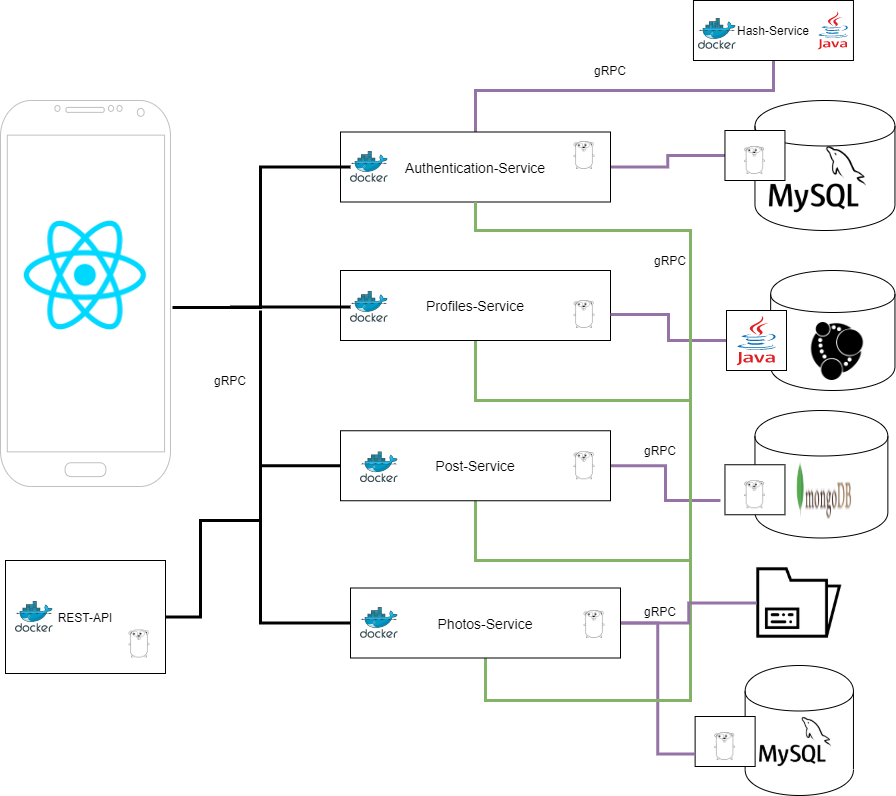
\includegraphics[width=120mm,scale=1]{img/main-uml.png}
		\caption{Application -  UML.}
		\label{application:uml}
	\end{center}
\end{figure}

\section{Objectives}
\vskip 0.1in
\indent
\indent
We expect to learn and prepare to afront the professional software environment after doing this project. The main objective of this project is to learn as much as we can to be ready to start our professional path in the software industry. Some of the objectives that we expect to achieve by doing this project are:

\begin{itemize}
	\item Research and learn new technologies that are utilized in the software industry.
	
	\item Apply agile techniques to develop an application based on initial requirements.
	
   	\item 	Develop a scalable microservices distributed system to manage a dynamically growing database. 
	
	\item Implement the system on the internet using the most popular cloud providers.
	Develop an application that efficiently works with images.
	
	\item Implement a reliable authentication system that securely stores passwords using hash and salt.
	
	\item Develop a high-performance mobile application that integrates the microservices.
	
	\item Develop a REST API that integrates the microservices.
	
	\item Works in a team utilizing flourishing software development tools.
\end{itemize}


\section{Design overview}
\indent
\indent
In this project, we utilize cutting-edge technologies to develop a micro-service application.   The application is developed using relational, document base, and graph databases. We look at the benefits of each database, and we use them where we can maximize performance base on how the data is store and access on each type of database.

The advantages that we want from developing the application as a distributed system are \cite{dsbook}:

\begin{itemize}
	\item Avoid expensive queries for fast performance. We use multiples databases to store the data in a simple way that makes access very fast. We avoid joins and any expensive query.
	
	\item	Scalability, each component performs a specific task; more instances of each service can be added.
	
	\item	Flexibility, each service is independent and composed of independents components as well; more components to perform a different task can be added on each service can be added, and new services can be created for a completely new task.
	
	\item Maintainability, services are easy to maintain because they are encapsulated and perform simple tasks.
	
\end{itemize}



\subsection{The Solution}
\indent
\indent
We have designed a tourism application where users create the data.  It stores data about three main types: users, cities, and places; all three have a public profile(public to register users of the application). Users create the cities and the places, and they can be created only once. Cities and places have a profile where users can post. Users can mark Cities and places as visited, so they will show in their profiles and have actualization about recent posts.

\paragraph{The principal user interfaces in the client are:}

\begin{itemize}
	\item User profile, which shows visited places and visited cities.
		\item Cities profile, which includes the places in the city and posts about the city.
	\item	Places profile, which includes posts about the place.
\end{itemize}

\subsection{The Microservices}

The application is divided into four main microservices:
\begin{itemize}
	\item The authentication service provides secure authentication storing passwords in binary format using hash and salt.
 \item	The profiles-service store primary data of all profiles.
\item	The post-service, store, and manage posts.
\item	The photo-service, manage, and stores photo for profiles and posts. 
\end{itemize}




\subsection{Databases Design}

Each service has its database. We have research best database that fits each of the services:
\begin{itemize}
	\item The authentication service uses a relational database. When a user login a token is generated, that token can be used to authenticate each request that the user performs. A leader/slave replication has been set up to improve performance. The read from the database is distributed on multiple databases to perform the most used operation that is to authenticate requests.
	
	\item	The profiles services use a graph database. We used the graph database to create relations that avoid complicated queries.
	
	\item The post-service use a document-based database. Posts are indexed and stored in scalable documents. We can use inexpensive queries to perform CRUD operations in the posts of a city or place.
	
	\item	The photo-service store images in the file system and use a relational database to store URLs. Binary images have public access from the file system, so the image is loaded directly from the client without the need to send the image through the service, the service store URL which is sent to the user.

\end{itemize}

\subsection{Technologies introduction}
\vskip 0.1in
\indent
\indent
After some research, we decide to use Goland as the main back end programing language; some parts of the system were also writing using Java. 

We have used gRPC as the communication interface for the microservices because it provides a transparent client/ server relation. We created a go module with all gRPC interfaces that can be imported in all the components of the application.

All the services are run using docker containers, and the images are published in Docker Hub and then pulled from virtual machines to run the service. 

We have work with the 3 most popular internet services providers(Azure, google cloud, and AWS), all of them offer free student credit, and we use that. In general, the 3 services have excellent performance and outstanding support, which was used several times to learn and fix errors.

We find that one of the best for us was google cloud because they live chat and convenient SSH on the browser.  Also, the container optimized OS is outstanding to work with docker images. 


\subsection{Methodology}
\vskip 0.1in
\indent
\indent
The project has been developed in an iterative approach based on agile principles, based on the original principles we have created an adaptation to feet the demands of our project.

We define stages that are reviewed during all the project development, measure progress based on the working code, continuously meet with the team, and be ready to adapt to any change in circumstances.

The solution was created component by component, integrating them after several independent testing, we keep a working solution all the time to which we integrate more components as they are developed.

\subsection{Context}
\vskip 0.1in
\indent
\indent
In Chapter 2, we explain the methodology used to develop the project. Chapter 3 is a technology review, where we research and decide the best technologies to use in each component for then have an in-depth look at them. In Chapter 4, we explain the full system design and the design of each element. Chapter 5 is the evaluation of the system; we show how it works and test it. And finally, in chapter 6, we provide a conclusion where we look at the achieved goals and possible future work.



 
  \chapter{Methodology}

\indent
\indent
In this section, we describe how we develop the project, we set our basis on the start, and them follow them during the development of the project. 

The section is divided in Back-end and Front-End because there where slightly different approaches in the developing process.
\section{Back-End}
Jose I. Retamal
\vskip 0.1in
\indent
\indent
Most successful software projects are developed using some agile methodology\cite{agilemanifesto}. There is a reason for this and is because the software is an intellectual product that needs to adapt to change on requirements, libraries, and hardware. This constant change required adaptative and iterative approaches to develop.

We adapted some of the agile principles to our project \cite{agilemanifesto}:
\begin{itemize}
	\item Continuous delivery. The application is tested at all stages, and we keep a working application all the time.
	\item Adapt to changes at any stage. Even if we started with a design and chose the technologies to be use, they can change at any stage. 
   	\item 	Work together with all participants. We continuously meet with all people involved in the project, check the stage of the project, and check if there is anything that needs to change.
	\item	Self-motivation. There is a personal interest in the project to all participants.
	\item	Working software is the measure of the stage of the project. What is done and working in the software is the main reference point on at what stage we are on the project.
	Simplicity. We develop a working application most simply, but without leaving the performance aside.
	\item	Self-organizing. Everyone in the project organizes himself in the way they think it would be the best way to have a maximum amount of productivity. 
\end{itemize}



\subsubsection{Stages of the Project}

There where three stages in the development of the application. They are not a hard stage, and they overlap each other(Figure \ref{methodology:stages}). These stages are a reference to know what to do, and they are regularly reviewed.

\begin{itemize}
	\item System Design.
	\item Technology Research.
	\item Implementation.
\end{itemize}

\begin{figure}
	\begin{center}
		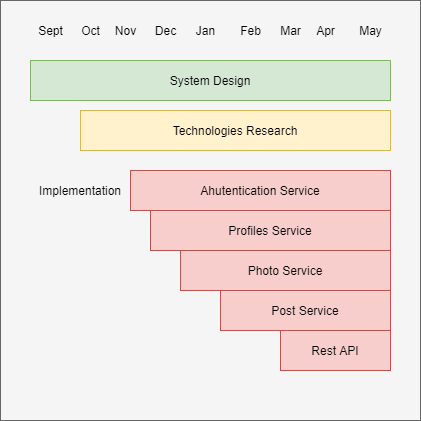
\includegraphics[width=120mm,scale=1]{img/metodology/gueneral-gant.png}
		\caption{Methodology- Project Gueneral Gant Chart.}
		\label{methodology:stages}
	\end{center}
	
\end{figure}

\paragraph{System Design}

We create a simple design of the system at the start. This defines, in a general way, the main components of the system. This was a quick process, and the design was always subject to updates.
To design the system, first, the requirements where set. Then the design was done following them.


\begin{itemize}
	\item Design the full system in a general way, understand more or less the number of services required.
	\item Define the function of each component.
	
\end{itemize}


\paragraph{Technology Research}

After we have an idea of the system, some time was spent on looking for the best technologies that will suit the application, some prototypes where design to check if they work.

\begin{itemize}
	\item Decide the main technologies to be used.
	\item	Test compatibility. 
\end{itemize}



\paragraph{ Implementation}

The implementation has been done using an iterative process. Starting from the authentication service, the system was build block by block. After one component was developed, it was tested to check that the full system works. 

On each component, we start by designing the database, the DBA, and then the main service with the endpoint to the client.

When starting to develop a new component, the full system design has to be check.


\subsection{System Development life cycle}
\indent
\indent
Each component is developed iteratively after some functionality is implemented the component is first tested locally, them docker images is created ann updated to docker hub, them the image is downloaded in the server, and the whole system is tested. The life cycle steps are below(Figure \ref{methodology:cycle}):

\begin{itemize}
	\item Build and test the component locally.
	\item Create/update a docker image and update it to the docker hub.
	\item Pull from docker hub, run the component in the network, and test.
	\item Test the full system. 
\end{itemize}


\begin{figure}
	\begin{center}
		\includegraphics[width=120mm,scale=1]{img/metodology/component-teration.png}
		\caption{Methodology- Component Iteration.}
		\label{methodology:cycle}
	\end{center}
	
\end{figure}

\subsection{Selection Criteria}
\label{sel:criteria}
\indent
\indent
We have applied the following criteria to chose the technologies used in the project.
\begin{itemize}
	
	
	\item Accessibility. Technologies must be accessible without a cost; they can be free and open-source or offer student free usage.
	\item New to us. One of the ideas of the project is to learn how to work with new technologies and learn. So we look for technologies that are not familiar to us.
	
	\item Popular and used in 
	They are professionally used. We want to learn how to use technologies that are popular and used in professional software development.
	
	\item Mature and recognized. We prefer technologies with background and maintained/developed by a recognized organization or a big open source community. Even if there are always new technologies coming out, we prefer those that are already established.
	
	\item It adapts well to the purpose need in the system.
	Simple and with resources to learn. We need to learn the technologies, so we instead chose those that are fast to learn and with many resources(tutorials and documentation) to access.
\end{itemize}

\subsection{ Testing}
\indent
\indent
Because of the time frame, we do not develop the application using automated testing. We know there are many advantages to it, but we need to trade off this feature. Some aspects that we considered to decide that automated testing is not for the project:
Most of the benefits of automated testing are long time benefits.
Automatested testing is practical another application that needs to be maintained.

Instead, based on the principle of self-motivated development, we develop the project using a test culture that relies on developers:
Each functionality needs to be tested by the developer at developing time.
Bugs found needs to be personally reported to the developer.
When integrating new components, the full system needs to be checked. 

\subsection{Security considerations for authentication}
\begin{itemize}

	\item  Feedback for password strength.
	\item  hash+ salt using bcrypt function on server and client.
	\item constant time function for compare hashed passwords.
\end{itemize}
\subsection{Tools}



\subsubsection{Integrated development environment}

\begin{itemize}

	\item  Eclipse for Java development. Solid IDE with just the right performance, we choose it because its well knows for us and free to use (\url{https://www.eclipse.org/}).
	\item  Goland, for Go development. Excellent IDE is free for students(\url{https://www.jetbrains.com/go/}). 
	\item  Visual Studio Code, general code review, and write docker images(\url{https://code.visualstudio.com/}).

\end{itemize}
\subsubsection{SHH Client}
\begin{itemize}
	
	\item  Putty, free shh client, open-source, and simple to use(\url{https://www.putty.org/}).
\end{itemize}

\subsubsection{Version Management}
\begin{itemize}
\item  Git, very popular with string community, we use the prevalent GitHub server(\url{https://git-scm.com/}). 
\item  Docker Hub, Manage containers, free for public containers (\url{https://hub.docker.com/}). 
\end{itemize}


  \chapter{Technology Review}

\section{Technologie Research and Decision }

\subsection{Ahutentication Service Database}
Jose I. Retamal
\vskip 0.1in
\indent
\indent

We need a database on where the data can be accessed quickly and reliably by index. We are also looking for a database that can be replicated. A relational SQL database fits the requirements. From MariaDB, MySQL, PostgreSQL, and oracle. MySQL and PostgresSQL have been selected for further analysis.

\subsubsection{MySql}

\paragraph{MySQL 5.6 \cite{lbpcmysql}}  
\paragraph{Pros} 
\begin{itemize}
\item Oracle has brought more investment into MySQL, meaning there is a future with it.
 \item It is a solid product. MySQL 5.6 is a reliable product with all the features fully tested.

\item There are many teams from Oracle working in MySQL.
\end{itemize}

\paragraph{Cons}

\begin{itemize}

\item Not so mature as other relations databases like PostgreSQL. This means that it has fewer features than the other more mature database systems.
\item  Not fully open source anymore, in theory, is open source, but in practice, Oracle has taken over. 
\item Many have replaced MySQL for MariaDB. Since oracle takes over MySQL, many big names like RedHat Enterprise Linux, Fedora, have moved to MariaDB.
\end{itemize}
\paragraph{ PostgreSQL \cite{sdpost}} 

\paragraph{Pros}

\begin{itemize}
\item Reach libraries for transactions. Fully documented with comments made it easy to know what part of the code does what and how it is done.
\item  Many adjustable parameters make the system easier to personalize. 
\item Easy to extend, if extra features are needed is possible to add the feature. Secure and reliable, also security can be personalized and extendible.
\end{itemize}
\paragraph{Cons}

\begin{itemize}
\item Open source, not owned for any organization that takes care of it. 
\item Slow performance, there have been reported issues with performance and backup recovery.
\end{itemize}


\paragraph{Conclusion}

\indent
\indent
There is not a real need for a feature-rich database; the database that we need to implement is simple, and the main aspect to consider is the replication—also, some of the cons of MySQL that be considered as advantages. Because MySQL is robust and has all the functionality needed, it has been chosen as the best option.


About seven to ten pages.
\begin{itemize}
\item Describe each of the technologies you used at a conceptual level. Standards, Database Model (e.g. MongoDB, CouchDB), XMl, WSDL, JSON, JAXP.
\item Use references (IEEE format, e.g. [1]), Books, Papers, URLs (timestamp) – sources should be authoritative. 
\end{itemize}

\section{XML}
Here's some nicely formatted XML:
\begin{minted}{xml}
<this>
  <looks lookswhat="good">
    Good
  </looks>
</this>
\end{minted}

  
\chapter{System Design}

\section{Ahuthentication Service}{Jose I. Retamal }



\indent
\indent
This service provides user authentication. It is composed of three components: the hash service, the database, and the main service (Figure \ref{auth:xxdfdfdfdf}).

The password is store securely, is hashed and salted using the hash service and then the hash and salt is stored in the database.

The database is replicated using the master follower topology. Create, update, and delete operations are always performed in the master, read operations are performed in followers. 

\begin{figure}[H]
\begin{center}
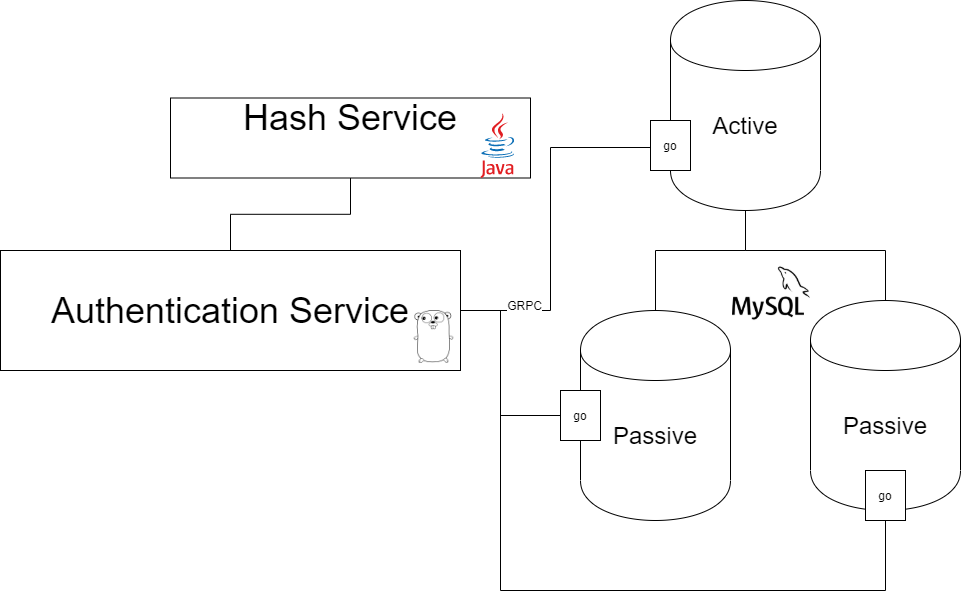
\includegraphics[width=120mm,scale=1]{img/auth/auth-main-uml.png}
\caption{Authentication Service- UML.}
\label{auth:xxdfdfdfdf}
\end{center}

\end{figure}


\subsection{Database Replication}

\indent
\indent
Replication it has been set up using MySQL 5.7 (See Appendix \ref{appendix:SetupReplication}),  we have set up a master and a replicate running in different Virtual Machine using Azure services. Using the instruction in Appendix \ref{appendix:SetupReplication} is possible to add more followers, for do tables in master need to be locked for a few minutes.

The load balancing is done using Round Robin, and standards go grpc librarie. helps in performance because the most used operation is to get user data or token to check authentication.

Is implemented as client-side replication, the client chooses a server one at the time to make the calls, the client in this situation is the authentication service, and the server is the authentication dba. The load balancing is implemented in the authentication service(Figure \ref{auth:createusersequence}).

\begin{figure}[h]
	\begin{center}
		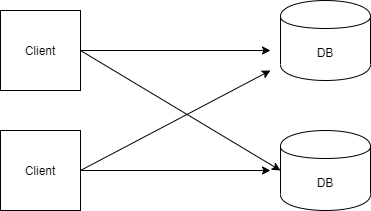
\includegraphics[width=90mm,scale=1]{img/auth/client-side-load-balancer.png}
		\caption{Authentication Service- Create User Sequence Diagram.}
		\label{auth:loadbalancerdiagram}
	\end{center}
\end{figure}

\subsection{Endpoints} 

\subsubsection{Create User}

\indent
\indent
Users create an account, and when this happens, a new entry is created in the authentication database. Also, a new entry is created in the profiles database (Figure   \ref{auth:createusersequence}). To create a user, this service needs to communicate with the profiles service.



\begin{figure}
\begin{center}
	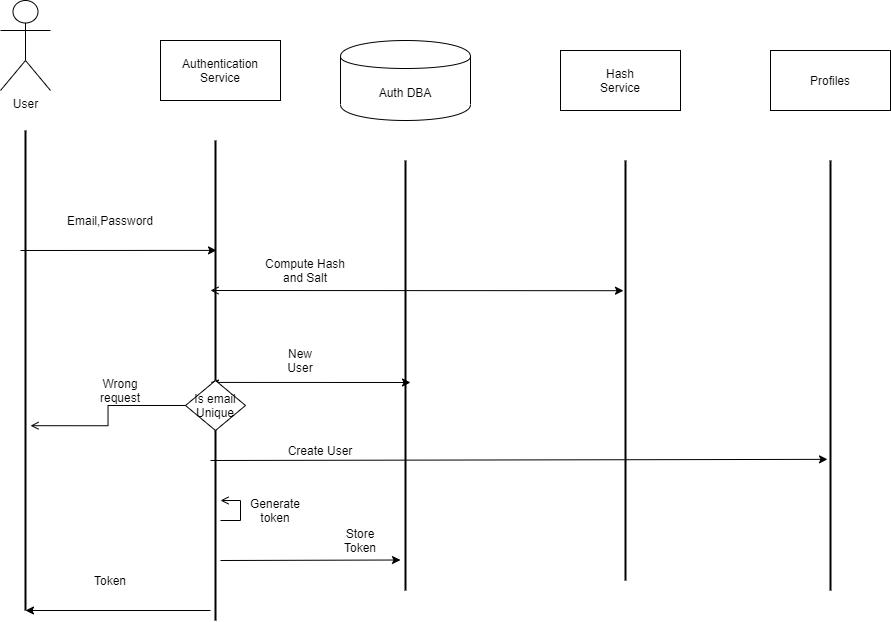
\includegraphics[width=90mm,scale=1]{img/auth/CreateUser_sequence.png}
	\caption{Authentication Service- Create User Sequence Diagram.}
	\label{auth:createusersequence}
\end{center}
\end{figure}

\subsubsection{Login user}
\indent
\indent
To login a user, we perform the followings steps (Figure \ref{auth:loginsequence}):
\begin{itemize}

\item Get user data from the authentication database.
\item	Check the password using the hash service.
\item	If the password is valid will generate a unique token, it stores the token in the database and sends the response to the client.
\end{itemize}

\begin{figure}
\begin{center}
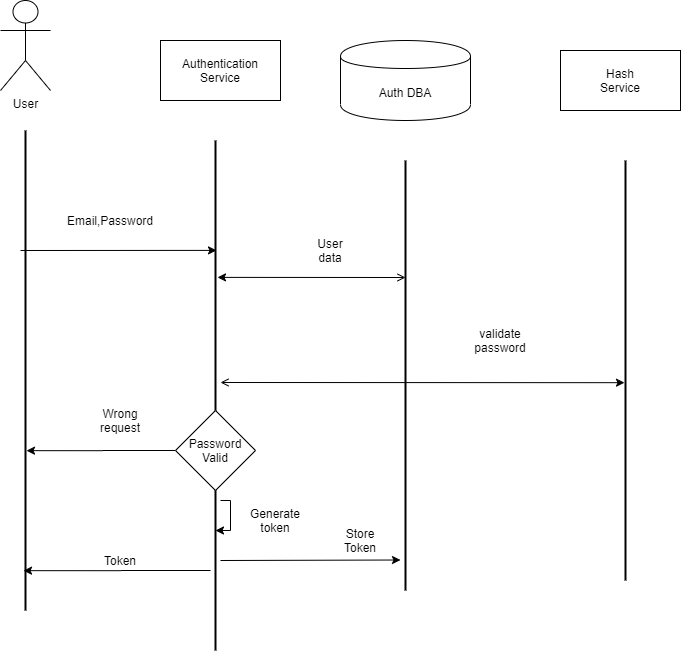
\includegraphics[width=90mm,scale=1]{img/auth/login-sequence.png}
\caption{Authentication Service- Login Sequence Diagram.}
\label{auth:loginsequence}
\end{center}

\end{figure}


\subsubsection{Check Token}

\indent
\indent
The most used endpoint, here is where replication plays a role for fast checking tokens. This is used in the most requests to all services to ensure security across the application (Figure \ref{auth:checktokensequence}).


\begin{figure}
\begin{center}
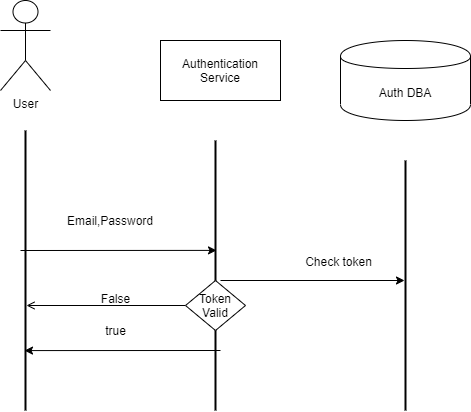
\includegraphics[width=90mm,scale=1]{img/auth/check-token-sequence.png}
\caption{Authentication Service- Check Token Sequence Diagram.}
\label{auth:checktokensequence}
\end{center}
\end{figure}

\subsubsection{Log out}
\indent
\indent
The request includes the token, and that token is removed from the sessions table in the authentication database.


\subsection{Authentication DBA}
\indent
\indent
This program provides access to the authentications database. Is written in go and runs in a docker container, it connects to a MySQL database running in localhost. The application communicates with the main authentication service through a grpc interface.

\subsubsection{The database}


\begin{figure}
\begin{center}
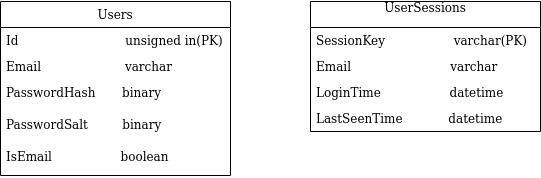
\includegraphics[width=90mm,scale=1]{img/auth/auth-db.png}
\caption{Authentication DBA- Authentication Database.}
\label{auth:authdbuml}
\end{center}

\end{figure}

\indent
\indent
The authentication database store the necessary user data for authentication and login.

 It is composed of two tables: the authentication table and the sessions table. The authentication table contains the user name, the password hash, and the password salt(Figure \ref{auth:authdbuml}).
 
  The user name is the email and is the unique identifier for all the systems, is not the primary key of the database, but is indexed for quick access. For this database, an extra integer field is added as the primary key. The password hash and salt are 32 bytes binaries strings. The sessions table uses a unique session key as a primary key for a quick check if a session exists. 
  
  When a user login a session is created and stored in this table. The user then can log in to the application using that session. When the user logs out, the session is deleted from the database.


\subsubsection{Endpoints}
\begin{itemize}
\item AddUser() : Create a new user in the database. When the user creates the account, it will create the profile automatically in the profiles database.

\item GetUser(): Returns the user data used to authenticate the user.

\item UpdateUser(): Update the user data, is used for changing the password.

\item CreateSeassion(): Create a new session in the database. Used when the user login  using the password.

\item GetSeassion() : Return a user session if exist. Used to check if the session exists so the user can log in without the password.

\item DeleteSession : Delete user session if exits. Used when the user logs out from the device.

\end{itemize}

\subsection{The Hash Service}

\indent
\indent
This service creates a password salted password hash using a randomly generated salt. It has been adapted from a Distributed Systems project from semester 7.
It checks the password in fix amount of time for security reasons. Attackers can guess passwords guess by comparing the time it takes to validate a password.
\newpage

As many pages as needed.
\begin{itemize}
\item Architecture, UML etc. An overview of the different components of the system. Diagrams etc… Screen shots etc.
\end{itemize}

\begin{table}[h]
  \centering
  \begin{tabular}{x{2cm}p{3cm}}
    \toprule \\
    Column 1 & Column 2 \\
    \midrule \\
    Rows 2.1 & Row 2.2 \\
    \bottomrule
  \end{tabular}
  \caption{A table.}
  \label{table:mytable}
\end{table}
  \chapter{System Evaluation}
As many pages as needed.
\begin{itemize}
\item Prove that your software is robust. How? Testing etc. 
\item Use performance benchmarks (space and time) if algorithmic.
\item Measure the outcomes / outputs of your system / software against the objectives from the Introduction.
\item Highlight any limitations or opportuni-ties in your approach or technologies used.
\end{itemize}
  \chapter{Conclusion}
About three pages.

\begin{itemize}
\item Briefly summarise your context and ob-jectives (a few lines).
\item Highlight your findings from the evalua-tion section / chapter and any opportuni-ties identified.
\end{itemize}
  \bibliographystyle{ieeetr}
  \bibliography{bibliography}
    \begin{appendices}
  	\chapter{Docker}{Jose I. Retamal }

  
\section{Install Docker in Ubuntu Using Command Line}	
  	
  
\subsection{Setup repository}
\begin{itemize}
\item Update packages 
	
\begin{minted}[linenos,tabsize=2,breaklines]{bash}
$ sudo apt-get update
\end{minted}

\item Install packages to allow apt to use a repository over HTTPS:

\begin{minted}[linenos,tabsize=2,breaklines]{bash}
$ sudo apt-get install \
	apt-transport-https \
	ca-certificates \
	curl \
	gnupg-agent \
	software-properties-common
\end{minted}

\item Add Docker’s official GPG key :
\begin{minted}[linenos,tabsize=2,breaklines]{bash}
$ curl -fsSL https://download.docker.com/linux/ubuntu/gpg | sudo apt-key add -software-properties-common
\end{minted}


\item Verify that you now have the key with the fingerprint 9DC8 5822 9FC7 DD38 854A E2D8 8D81 803C 0EBF CD88, by searching for the last 8 characters of the fingerprint.
\begin{minted}[linenos,tabsize=2,breaklines]{bash}
$ sudo apt-key fingerprint 0EBFCD88
\end{minted}


\item set up the stable repository:
\begin{minted}[linenos,tabsize=2,breaklines]{bash}
$ sudo add-apt-repository \
	"deb [arch=amd64] https://download.docker.com/linux/ubuntu \
	$(lsb_release -cs) \
	stable"
\end{minted}

\end{itemize}

\subsection{Install Docker Community}

\begin{itemize}
	
	\item Install the latest version of Docker Engine - Community and container, or go to the next step to install a specific version:
	\begin{minted}[linenos,tabsize=2,breaklines]{bash}
	$ sudo apt-get install docker-ce docker-ce-cli containerd.io
	\end{minted}
	
	\item Verify that Docker Engine - Community is installed correctly by running the hello-world image.
	\begin{minted}[linenos,tabsize=2,breaklines]{bash}
	$ sudo docker run hello-world
	\end{minted}
	
\end{itemize}


\section{Run Image Using Docker Hub}	

\begin{itemize}
\item  Create repository in Docker Hub.

https://docs.docker.com/docker-hub/repos/
\item  Build Image (Local machine):
	
\begin{minted}[linenos,tabsize=2,breaklines]{bash}
$ sudo docker image build -t docker-hub-user-name/image-name:version-tag .  
\end{minted}

Example:

\begin{minted}[linenos,tabsize=2,breaklines]{bash}
$ sudo docker image build -t joseretamal/hash-service:1.0 . 
\end{minted}

\item  Push Image (Local machine):

\begin{minted}[linenos,tabsize=2,breaklines]{bash}
$ sudo docker push docker-hub-user-name/image-name:version-tag
\end{minted}

Example:

\begin{minted}[linenos,tabsize=2,breaklines]{bash}
$ sudo docker push  joseretamal/hash-service:1.0  
\end{minted}

\item  Pull Image (Remote machine):

\begin{minted}[linenos,tabsize=2,breaklines]{bash}
$ sudo docker pull docker-hub-user-name/image-name:version-tag  
\end{minted}

Example:

\begin{minted}[linenos,tabsize=2,breaklines]{bash}
$ sudo docker pull joseretamal/hash-service:1.0  
\end{minted}

\item  Run image (Remote machine):

\subitem Opening a port and restart on crash or reboot:
\begin{minted}[linenos,tabsize=2,breaklines]{bash}
$ sudo docker run -d -p internal-port:open-port --restart always --name instance-name user-name/image-name:version-tag  
\end{minted}
Example:
\begin{minted}[linenos,tabsize=2,breaklines]{bash}
$ sudo docker run -d -p 5151:5151 --restart always --name hash-service joseretamal/hash-service:1.0  
\end{minted}

\subitem Allowing instance to full network acess (allows acess to local host):
\begin{minted}[linenos,tabsize=2,breaklines]{bash}
$ sudo docker run -d -p  --network="host" --restart always --name instance-name  user-name/image-name:version-tag 
\end{minted}
Example:
\begin{minted}[linenos,tabsize=2,breaklines]{bash}
$ sudo docker run -d -p  --network="host" --restart always --name hash-service joseretamal/hash-service:1.0 
\end{minted}

\item Stop instance: (Remote machine):

\begin{minted}[linenos,tabsize=2,breaklines]{bash}
$ sudo docker rm --force instance-name
\end{minted}
Example:
\begin{minted}[linenos,tabsize=2,breaklines]{bash}
$ sudo docker rm --force hash-service
\end{minted}

\item Check logs: (Remote machine):

\begin{minted}[linenos,tabsize=2,breaklines]{bash}
$ sudo docker logs instance-name
\end{minted}
Example:
\begin{minted}[linenos,tabsize=2,breaklines]{bash}
$ sudo docker logs hash-service
\end{minted}

\item Bash into the container: (Remote machine):

\begin{minted}[linenos,tabsize=2,breaklines]{bash}
$ sudo docker exec -it instance-name bash
\end{minted}
Example:
\begin{minted}[linenos,tabsize=2,breaklines]{bash}
$ sudo docker exec -it hash-service bash
\end{minted}

\end{itemize}
	
  	\chapter{MySql}
Jose I. Retamal
\vskip 0.1in
\indent
\indent

\section{Install Mysql in Linux Using Command Line}	


\subsection{Install MySQL-shell}

\begin{itemize}
	
\item Make sure you do not skip the step for updating package information for the MySQL APT repository: 
	
	\begin{minted}[linenos,tabsize=2,breaklines]{bash}
	$ sudo apt-get update
	\end{minted}
	
	\item Install MySQL Shell with this command: 
	
	\begin{minted}[linenos,tabsize=2,breaklines]{bash}
	$ sudo apt-get install mysql-shell
	\end{minted}
\end{itemize}

\subsection{Install MySql server}

\begin{itemize}
	

	
	\begin{minted}[linenos,tabsize=2,breaklines]{bash}
	$ sudo apt-get install mysql-server
	\end{minted}
	

\end{itemize}

\subsection{Uninstall MySql server}

\begin{itemize}
	
	
	
	\begin{minted}[linenos,tabsize=2,breaklines]{bash}
	$ sudo apt-get remove --purge mysql*
	$ sudo apt-get purge mysql*
	$ sudo apt-get autoremove
	$ sudo apt-get autoclean
	$  sudo apt-get remove dbconfig-mysql
	$ sudo apt-get dist-upgrade
	\end{minted}
	
	
\end{itemize}

\subsection{Setup Replication}
\label{appendix:SetupReplication}

https://www.digitalocean.com/community/tutorials/how-to-set-up-master-slave-replication-in-mysql

\subsubsection{setup master}

\begin{itemize}
	
	
	\item Edit the mysql config file,for open the file using vi:
	
	\begin{minted}[linenos,tabsize=2,breaklines]{bash}
	$sudo vi /etc/mysql/mysql.conf.d/mysqld.cnf
	\end{minted}
	\item make the followings changes to the the file, if the field are missing they must be added or if they are commented un commented:
	\begin{minted}[linenos,tabsize=2,breaklines]{bash}
	server-id       = 1
	log_bin                 = /var/log/mysql/mysql-bin.log
	binlog_do_db  = replica1
	sudo mysql_secure_installation
	\end{minted}
	
	\item Restart MySQL:
		\begin{minted}[linenos,tabsize=2,breaklines]{bash}
	$ sudo service mysql restart
	\end{minted}
	
	\item Create user for replication and give permissions:
		\begin{minted}[linenos,tabsize=2,breaklines]{bash}
	$ sudo mysql -u root
	mysql>GRANT REPLICATION SLAVE ON *.* TO 'slave_user'@'%' IDENTIFIED BY 'password';
	FLUSH PRIVILEGES;
	\end{minted}
	
	\item Get master status, after select the database in one MySQL seasiion :
			\begin{minted}[linenos,tabsize=2,breaklines]{bash}
	 mysql>FLUSH TABLES WITH READ LOCK;
	\end{minted}
	
	\item then open another MySQL seasion(keep the other open):
	
	\item Get master status, after select the database in one MySQL seasiion :
	\begin{minted}[tabsize=2,breaklines]{bash}
	mysql>SHOW MASTER STATUS;
	| File             | Position | Binlog_Do_DB | 
	+------------------+----------+--------------+--
	| mysql-bin.0001580 |      154 | user_login   |          
	+------------------+----------+--------------+----
	\end{minted}
	
	Note the file (mysql-bin-0001580) and the position.
	
	\item After take note of file name and position  tables can be unlocked :
	\begin{minted}[linenos,tabsize=2,breaklines]{bash}
	mysql>UNLOCK TABLES;
	\end{minted}
	
	\subsubsection{setup slave}
	
	\item Edit slave config file :
	\begin{minted}[linenos,tabsize=2,breaklines]{bash}
	$ sudo vi /etc/mysql/my.cnf
	\end{minted}
		
	Make the following modifications:
	
	\begin{minted}[linenos,tabsize=2,breaklines]{bash}
	server-id               = 2
	relay-log               = /var/log/mysql/mysql-relay-bin.log
	log_bin                 = /var/log/mysql/mysql-bin.log
	binlog_do_db            = newdatabase
	\end{minted}
	
	\item Restart MySQL service :
	\begin{minted}[linenos,tabsize=2,breaklines]{bash}
	$ sudo service mysql restart
	
	\end{minted}
			\item Config slave in mysql shell:
	\begin{minted}[linenos,tabsize=2,breaklines]{bash}
		mysql> CHANGE MASTER TO
		MASTER_HOST='104.40.206.141',
		MASTER_USER='repl',
		MASTER_PASSWORD='password',
		MASTER_LOG_FILE='mysql-bin.000160',
		MASTER_LOG_POS= 2439;
		\end{minted}
	
	\item Start slave
	\begin{minted}[linenos,tabsize=2,breaklines]{bash}
	mysql> START SLAVE;
		\end{minted}
	
	\item Check status
	\begin{minted}[linenos,tabsize=2,breaklines]{bash}
	mysql> SHOW SLAVE STATUS\G
	\end{minted}
	
\end{itemize}

  \end{appendices}

\end{document}
